
\section{Agents and Agent Based Modeling in Cyclus}\label{abm:abm}

Deciding how a simulation is structured from an interactions standpoint is a
delicate balance of known necessity and perceived future needs. There are basic
decisions to make, such as modeling material transfer as discrete or
continuous. Discrete transfers more closely match reality and may provide
insights in that regard, however they require more of their modeling apparatus
due to messaging needs and other structures. More complex decisions include how
one wants to determine connections between facilities, and whether such
connections are assigned statically and incorporated into the simulation
architecture or determined dynamically. Guerin's comment
in \S\ref{sec:litrev-benchmarks} stems from this ``freedom''. These
simulation-engine decisions comprise the art-related portion of fuel cycle
simulation, but developers have a goal of making these decisions in as informed
a way as possible using domain-level knowledge with respect to our known and
perceived requirements. In general, this work tries to minimize the sheer number
of choices we make in this regard, instead relying on well known and well
documented practices of computer scientists and systems engineers.

The \Cyclus team is also interested in fostering a user and developer ecosystem.
Accordingly, such concerns also drive the simulation architecture design. The
agent-based nature of \Cyclus provides an opportunity to reduce barriers to
entry into the ecosystem. Given a few basic tenets of agent interaction, other
developers should be able to create a new agent to ``plug in'' to the
simulation. Intuitively, a minimal set of behaviors must be defined to
sufficiently inform the simulation infrastructure to run the simulation. This
freedom allows the simulation program introduce agents at run time, effectively
separating the simulation engine's functionality from the agents in the
simulation.

Such a framework provides many benefits. First, there is a clear separation of
concerns. The \Cyclus core is concerned with modeling system dynamics whereas
individual agents are concerned with domain-specific issues. Accordingly,
developers can focus their attention appropriately, focusing either on the core
code base or on agent development. Separating agent development from core
development also allows \Cyclus to remain a viable open-source candidate to
model nuclear fuel cycle dynamics. Because domain-level information is
incorporated into agent libraries which are dynamically loaded at runtime, a
closed-source developer can focus their efforts entirely on developing agent
libraries. Furthermore, developers could participate both privately and
publicly, e.g., adding general capability to the \Cyclus core that is needed for
some functionality without specifying the internals. Such a community paradigm
is shown in Figure \ref{fig:community}.

\begin{figure}[htbp!]
  \begin{center}
    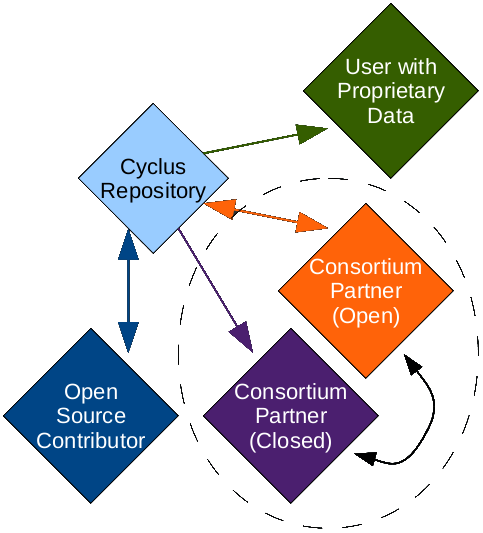
\includegraphics[height=8cm]{./figs/community.png}
  \end{center}
  \caption{The Cyclus Participation Paradigm} 
  \label{fig:community}
\end{figure}

In order to develop and maintain the core code separate from the agent modules,
well-defined interactions must be provided between agents and the \Cyclus
core. The remaining part of the section provides a proposal for such
interactions that allow for a variety facility deployment and supply-demand
matching algorithms to be employed. A description of the market resolution
interface is provided, and basic agent simulation interaction, such as entering
and leaving the simulation is also described.

Moving from a modeling paradigm that does not differentiate between individual
facilities to one that does requires a nuanced approach to determine facility
behavior. In the absence of supply constraints, aggregated individual facility
behavior and fleet-based models are equivalent. However, any system in which
recycling exists will, by definition, have some supply constraints. 

Furthermore, if resource supply and demand depends on more than the quantity of
a resource, moving global management logic becomes difficult. As the complexity
of a quality metric increases, an aggregate approach becomes less desireable as
it loses such detail through aggregation.

In the extreme in which a high level of detail is required in the notion of
resource quality, e.g. tracking an arbitrary number of isotopes, adopting
techniques that allow decision-making based on that level of detail is
desireable. Modeling the nuclear fuel cycle represents such a level of
detail. For example, even in the case of a once-through fuel cycle, many
reactors of the same type (e.g., PWRs), may require different resource qualities
(i.e., Uranium enrichment).

\subsection{Agent Taxonomy}

The Cyclus kernel implements a basic \code{Agent} class that provides the
minimal interface for agents to be built within a simualtion. Furthermore, the
\code{Trader} interface provides a communication layer required for agents to be
included in the exchange of resources. \code{Facility} agents in Cyclus
implement both interfaces, while \code{Institution} and \code{Region} agents
implement only the \code{Agent} interface.

\subsubsection{Facilities}

Facilities in \Cyclus are abstracted to either consumers or suppliers of
commodities, and some may be both. Supplier agents are provided agency by being
able to communicate to the market-resolution mechanism a variety of production
capacity constraints in second phase of the information gathering
methodology. Consumer agents are provided agency by being able to assign
preferences among possible suppliers based on the supplier's quality of
product. Because this agency is encapsulated for each agent, it is possible to
define strategies that can be attached or detached to the agents at
run-time. Such strategies are an example of the Strategy design pattern
\cite{vlissides_design_1995}.

\subsubsection{Institutions}

Institutions in \Cyclus manage a set of facilities. Facility management is
nominally split into two main categories: the commissioning and decommissioning
of facilities and supply-demand association. The goal of including a notion of
institutions is to allow an increased level of detail when investigating
regional-specific scenarios. For example, a consumer facility may prefer to be
supplied by a supplier facility in its instution rather than one associated with
a different institution. Furthermore, there are international governmental
organizations, such as the IAEA, that have proposed managing large fuel cycle
facilities that service many countries in a given global region. A fuel bank is
an example of such a facility. Accordingly, institutions in \Cyclus are able to
augment the preferences of supplier-consumer pairs that have been established in
order to simulate a mutual preference to trade material within an
institution. Of course, situations arise in real life where an institution has
the capability to service its own facilities, but choose to use an outside
provider because of either cost or time constraints. Such a situation is allowed
in this framework as well. It is not clear how such a relationship should be
instantiated and to what degree institutions should be allowed to affect their
managed facilities' preferences. This issue lies squarely in the realm of
simulation design decisions, part of the \textit{art} of
simulation. Accordingly, through the course of research, the possible design
space will be analyzed in order to determine best practices for this type of
design.

\subsubsection{Regions}

Regions in \Cyclus provide the forcing function for simulations by requiring
that certain parameters be met, e.g., power capacity, fuel cycle service
capacity, etc. For example, in the case of nuclear power capacity, a region
knows that it needs additional reactors to be built, but leaves the building of
those reactors to the institutions that operate in the region. The current
GrowthRegion model in the \Cycamore \cite{cycamore2013} code base takes the cost
and nameplate capacity for each facility in a set of acceptable facilities and a
demand gap, and solves a minimum-cost capacity production problem to determine
the number and type of facilities to request. It is important to note here that
this abstraction allows for different deployment algorithms to be tested and
exchanged in the \Cyclus framework without necessitating changes to the
simulation engine, as is the case with other simulators described
in \S\ref{sec:simulators} and is consistent with the types of simulation design
decisions described in
\S\ref{sec:simulators-overview}. 

Regions are further provided agency by their ability to affect preferences
between supplier-consumer facility pairs in the third phase of the market
information gathering algorithm. The ability to perturb arc preferences between
a given supplier and a given consumer allows fuel cycle simulation developers to
model relatively complex interactions at a regional level, such as tariffs and
sanctions. Constraints to cross-border trading can also be applied to the
formulation described in \S\ref{sec:gfctp}. For example, a region could place
constraints on the total amount of a given commodity type that is able to flow
into it or out of it into a different region. Such constraints could applied not
only to bulk quantities of a commodity, but also to the quality of each
commodity. Such a mechanism could be used to model interdiction of
highly-enriched uranium transport, for example.

\subsection{Methods of Agency}

Agency is provided in two primary modes: determining facility deployment and
informing resource exchange mechanisms. 

Facility deployment has, to date, involved some combination of an
\code{Institution} agent, a \code{Facility} agent, and a \code{Region}
agent. \code{Institution} agents represent a simulation entity abstraction that
can deploy \code{Facility} agents. \code{Region} agents represent a simulation
entity abstraction that have a demand for certain commodities that
\code{Facility} agents provide, for example, reactor-like \code{Facility} agents
provide electrical power.

\code{Facility} agents are further provided agency by informing market
mechanisms of thesupply and demand of resource quantity and quality. Cyclus
initially used a very crude interface and algorithm for determining resource
transactions. Individual markets were defined, and initially designed to be
agents much like \code{Facility}, \code{Institution}, and \code{Region}
agents. Many limitations were identified at the time, however, and this approach
was eventually abandoned. An enumeration of the observed limitations is
described further in \S \ref{abm:abm:limits}.

The Dynamic Resource Exchange (DRE), described in detail in \S \ref{abm:dre}, is
the mechanism eventually developed to drive supply-demand transactions. The
primary source of agency is provided to \code{Facility} agents in order to
negotiate the quanity and quality of potential resource
transactions. \code{Region}, \code{Instituion}, and \code{Facility} agents are
then provided agency in the negotiation of preferences of potential
transactions, where preference is a proxy for price.

\subsection{Proof of Principle}\label{abm:abm:proof}

Agents were developed to show an initial proof of principle that fuel cycle
simulation can be implemented using an agent-based modeling methodology.

Facility deployment decision making is the fundamental building block of any
dynamic simulator. By definition, dynamic simulators model the deployment of
facilities and measure the flow of resources in the system over time. 

Furthermore, in the extreme case of unconstrained supply and no competition for
resources, resource exchange decisions can be made arbitrarily. Therefore, only
facility deployment agency is required.

\subsubsection{Benchmark Case}

An initial benchmark test was performed to confirm expected deployment behavior
and basic resource routing. The INPRO Business As Usual (BAU) benchmark for the
once-through fuel cycle was chosen for three reasons. First, it was the simplest
case that demonstrated deployment behavior. Second, no supply or demand
constraints were present, so a basic supply-demand framework would
suffice. Finally, results from two other fuel cycle simulation codes, VISION
\cite{} and GENIUSv2 \cite{}, the predecessor of Cyclus, were available for
comparison. The INPRO BAU benchmark identified two cases, high electricity
demand and moderate electricity demand, as shown in
Fig. \ref{fig:inpro-demand}. Both cases require that demand met by a composition
of 94\% Light Water Reactors and 6\% Heavy Water Reactors.

\begin{figure}
  \begin{center}
    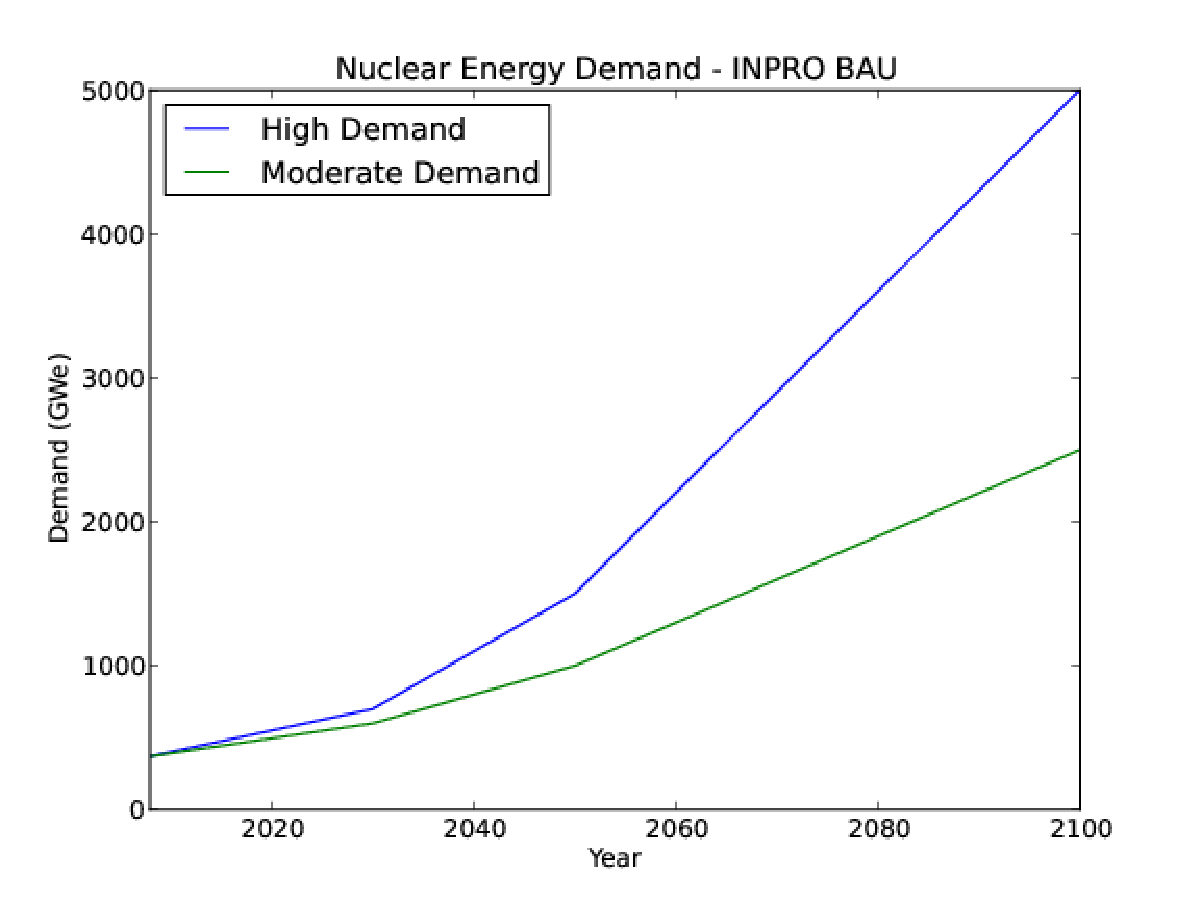
\includegraphics[height=8cm]{./figs/inpro-demand.pdf}
    \caption{The energy demand specification for the INRPO BAU scenarios.}
    \label{fig:inpro-demand}
  \end{center}  
\end{figure}

The goal of this proof-of-principle benchmark was to showcase the capability for
a developer to generate the required Facility, Institution, and Region
archetypes, and that such archetypes could be deployed in the Cyclus simulation
framework and generate satisfactory results. Metrics including deployment
patterns, natural uranium consumed, and used fuel produced by all reactors were
used to compare results between VISION, GENIUS, and Cyclus.

\subsubsection{Agent Archetypes Developed}

\paragraph{GrowthRegion}

The \code{GrowthRegion} was developed to assist in facility deployment
logic. The \code{GrowthRegion} takes as input a listing of commodities for which
it has a demand. For example, the The \code{GrowthRegion} agents in this
benchmark demand electrical power. The demand for commodities is defined by
symbolic functions. Currently, linear functions, exponential functions, and
piecewise combinations of both are supported. 

At any time step in which there exists a demand gap, i.e., there exists more
demand than supply, a build decision is made. This decision is modeled as the
following integer program:
%%%
\begin{subequations} \label{eqs:growth}
\begin{equation} \label{eq:optBuildObj}
\begin{aligned}
& \min
& & \sum_{i \in I}n_i*c_i
\end{aligned}
\end{equation}
\begin{equation} \label{eq:optBuildConst}
\begin{aligned}
& \text{s.t.}
& & \sum_{i \in I}n_i*\phi_i \ge \Phi
\end{aligned}
\end{equation}
\begin{equation} \label{eq:optBuildBounds}
\begin{aligned}
& n_i \in [0,\infty) & \forall \:\: i \in I &
\end{aligned}
\end{equation}
\begin{equation} \label{eq:optBuildInt}
\begin{aligned}
& n_i \:\:\: integer & \forall \:\: i \in I &
\end{aligned}
\end{equation}
where $\Phi$ is the unmet demand, $I$ is the set of facilities capable of 
meeting the demand, and, for each facility in $I$, $c_i$ is the cost of building, 
and $\phi_i$ is the nameplate capacity.  Finally, $n_i$ is the optimized number of
facilities to build of type $i$.
\end{subequations}
%%%

\paragraph{ManagerInst}

The \code{ManagerInst} was developed to assist in facility deployment as
well. While the \code{GrowthRegion} determines which facilities \textit{should}
be built, the \code{ManagerInst} determines the set of all possible facilities
that \textit{can} be built. In other word, the \code{ManagerInst} determines the
set of facilities, $I$, shown in in Eqn. \ref{eqs:growth}. Note that the set $I$
can change over time. Once a deployment decision is made, the
\code{GrowthRegion} makes a facility deployment request of the
\code{ManagerInst} which then deploys the chosen facility.

\paragraph{BatchReactor}

While a reactor model existed prior to this work, it did not provide the
functionality to interchange \textit{batches} of fuel. A batch of fuel is a
fraction of a full reactor core that is extracted and then replaced when a
reactor is refuled. While in the extreme, a full core can be replaced, in
pratice a batch size is generally a set fraction of the full core, especially
for LWRs.

The \code{BatchReactor} used in this work had configurable properties as
displayed in Table \ref{tbl:batchrxtr}. The values used based on the defined
INPRO BAU benchmark are described in Table \ref{tbl:inprorxtr}.

\begin{table}[ch]
\centering
\begin{tabular}{cc}
Parameter      & Description                     \\ \hline
Process Time   & Active fuel time in the reactor                        \\
Refuel Time    & Time to refuel the reactor                              \\
N Batches      & Number of batches in the reactor                         \\
Batch Size     & Quantity of a batch                                 \\
Power Capacity & Nameplace Capacity for Power                          \\
Power Cost     & Cost to build a new reactor      \\ \hline
\end{tabular}
\caption{Configurable input for the \code{BatchReactor} archetype.}
\label{tbl:batchrxtr}
\end{table}

\begin{table}[h]
\centering
\begin{tabular}{ccc}
Parameter      & LWR Values & HWR Values               \\ \hline
Process Time   & 10         & 10                       \\
Refuel Time    & 2          & 2                        \\
N Batches      & 4          & 4                        \\
Batch Size     & 7.87E4     & 1.39e5                   \\
Power Capacity & 1000       & 600                      \\
Power Cost     & 1000*      & 600* \\ \hline
\multicolumn{3}{l}{(*) Note that the Cost used is arbitrary and set equal to the
  capacity so that a minimum capacity is built per Eqn. \ref{eqs:growth}.}
\end{tabular}
\caption{Configurable input values for reactors used in the INPRO BAU once-through benchmark..}
\label{tbl:inprorxtr}
\end{table}

\paragraph{EnrichmentFacility}

\subsubsection{Results}

As designed, facility deployment curves match the required benchmark specification. 

Further, material transaction quantities match VISION values.

Enrichment values match VISION for SWU, however, tails values did not match.

(add more discussion and result images from ANS talk)

\subsection{Multiple Market Limitations}\label{abm:abm:limits}

Cyclus was originally designed to use an addition agent type, the \code{Market}
agent. The \code{Market} agents were envisioned to represent markets for
specific commodities. For example, the simulation described in \S
\ref{abm:abm:proof} used three commodity markets: natural uranium, enriched
uranium fuel, and used fuel. This approach is valid in the absence of supply or
demand constraints, competition, and fungibility. However, the inclusion of any
one of these features requires a much more involved process.

If supply or demand constraints are to be modeled, each
associated \code{Market} agent must have both a corresponding communication
interface and an implementation that accounts for such constraints. While
quantity constraints are not unreasonable to implement and support, quality
constraints are much more difficult. Furthermore, communicating such constraints
is difficult. Whereas the \code{Market} agent can implement a solver algorithm,
constraints are more naturally defined by the trader interacting with the
\code{Market} agent. For example, consider the enriched uranium market used in
\S \ref{abm:abm:proof}. While the simulation used an agent abstraction for an
enrichment facility and fuel fabrication plant, another simulation may wish to
model facilities that downblend HEU, rather than enrich LEU. Such a process will
have different constraints. Importantly, those constraints are a function of the
\code{Facility} agent, not of a \code{Market} agent.

Assuming that supply or demand is constrained either quantitatively or
qualitatively, competition for the resource in question can arise. In fact,
resources constraints are only interesting in the presence of competition. When
competition for resources exist, there must be some mechanism that determines
which transactions are to be executed, i.e., which agents should trade which
resources. Determining supply and demand under competition is a well studied
problem with many possible formulations and solution frameworks.

Fungibility is the property of a good or commodity to be \textit{capable of
  being substituted in place of one another} (CITE
http://www.merriam-webster.com/thesaurus/fungible). For example, a light water
reactor generates power by fissioning nuclei in the thermal energy
spectrum. Whether those nuclei are \nucl{239}{Pu}, \nucl{235}{U}, or
\nucl{233}{U} makes little difference from a power generation perspective. In
other words, those nuclei are \textit{fungible} for light water reactors, given
some safety and cycle length considerations. A similar issue arises from a
suppliers perspective. Consider a MOX fuel supplier and two requesters: a fast
reactor and a thermal reactor. Given the isotopic makeup of Plutonium in the MOX
fuel, such could be potentially be used in either reactor type. Again, Plutonium
in this example is a \textit{fungible} resource. Accordingly, a facility may
demand multiple fungible commodities, which must be accounted for by a given
market clearing mechanism.

The one-market-per-commodity approach does not treat competition, constrained
supply and demand, and fungibility particularly well. Constraints are handled
poorly because constraints are determined by the supplying and demanding
agents. Because the markets are separated, they must either be solved
sequentially or in parallel. If solved sequentially, competition and fungibility
are treated poorly, because information involving multiple commodities is not
taken into account during the solution of a single market. Accordingly, a
solution framework and methodology that incorporates agent querying of supply,
demand, and constraints and resolves markets in parallel is required.
